% !TeX program = pdflatex
% ISBI 2027 four-page paper. Style files: spconf.sty, IEEEbib.bst.
% Numbers come from experiments/label_prop{,_spread,_sam2_quartile,_sam2_spread,_sam2_one_mid,_sam2_two_third}
% experiments/cross_slice_ssl (masked modelling rows only), cross_cohort and nnunet_baseline. Before the SSL cut: main_v6_before_ssl_cut.tex.
\documentclass{article}
\usepackage[T1]{fontenc}
\usepackage{spconf,amsmath,graphicx}
\usepackage{enumitem}
\usepackage{booktabs}
\usepackage{url}
\usepackage{xcolor}
\graphicspath{{figures/}}
\setlist{nosep, leftmargin=14pt}
\newcommand{\todo}[1]{\textcolor{red}{[TODO: #1]}}

\title{One Annotated Slice per Mouse Suffices:\\Label Propagation for Brain Extraction in Preclinical MRI}

% TODO: confirm author list, order and affiliations with coauthors (copied from the previous paper).
\name{Tayyab Ali$^{\star}$, Xin Huang$^{\star}$, Miroslaw Janowski$^{\dagger}$, Guanda Qiao$^{\dagger}$, Lei Zhang$^{\star}$}
\address{$^{\star}$ Department of Computer and Information Sciences, Towson University, Towson, MD, USA\\
$^{\dagger}$ Department of Diagnostic Radiology and Nuclear Medicine,\\
University of Maryland School of Medicine, Baltimore, MD, USA}

\begin{document}
\maketitle

\begin{abstract}
Brain extraction is the first step of most preclinical MRI pipelines, and training a network for it still requires every slice of every mouse to be outlined by hand. We ask how few annotated slices per mouse are enough when the remaining slices receive automatically propagated labels. On 20 mice under animal-level five-fold cross-validation, we compare copying, shape-based interpolation, self-training, a registration network with an anchor-consistency loss and the video foundation model SAM2 as propagators. With three annotated slices per training mouse, a 2.5D network trained on SAM2-propagated labels reached a Dice of 0.950 and an HD95 of 8.9~px, against 0.946 and 9.0~px with every slice annotated. A single annotated slice per mouse, 9\% of all slices, gave 0.950 and was non-inferior to full annotation at a margin of 0.01 Dice ($p<0.001$), whereas training on that slice alone gave 0.891. The same held for nnU-Net, which reached 0.958 from one slice with SAM2 labels against 0.960 with full annotation. Copying or interpolating masks lowered accuracy below training on the annotated slices alone. Filtering propagated labels by agreement with an anchor-trained network improved registration but reduced SAM2 to 0.940, because SAM2 had labelled 78\% of the excluded pixels correctly against 60\% for registration.
\end{abstract}

\begin{keywords}
Brain extraction, mouse MRI, sparse annotation, label propagation, SAM2
\end{keywords}

\section{Introduction}
\label{sec:intro}

Preclinical neuroimaging pipelines typically begin with brain extraction, which is required before tasks such as atlas registration, volumetric analysis, and lesion assessment \cite{hsu2020skullstripping, defeo2021munet}. Although deep segmentation networks can perform brain extraction accurately, training them still depends on manually outlined masks. These masks are usually drawn slice by slice, making annotation one of the main bottlenecks when adapting a model to a new scanner, imaging protocol, or disease model. In our dataset, each mouse brain spans approximately 11 axial slices. Thus, even a relatively small training cohort of 14 mice requires more than 150 manual outlines.

Several approaches have been explored to reduce this annotation burden. One is self-supervised pretraining, which uses unlabelled images to learn useful representations before segmentation training. In our previous work, for example, masked image modelling improved a 2D U-Net for mouse brain extraction \cite{ali2025ssl}. Another approach is sparse annotation, in which only a subset of slices in each volume is labelled \cite{cicek2016unet3d}. Labels for the remaining slices can then be generated automatically, either by the segmentation network itself or through a separate propagation method.

Such propagation can be performed geometrically. Examples include shape-based interpolation \cite{raya1990shape} and deformable registration between neighbouring slices \cite{balakrishnan2019voxelmorph}. More recently, promptable foundation models have provided another option. SAM2, for instance, can track an object through a video when given a segmentation mask on one frame \cite{ravi2024sam2}. Medical adaptations have used the same idea by treating a stack of image slices as a video sequence \cite{ma2024medsam, zhu2024medicalsam2}. SLM-SAM~2 propagates annotations from a small number of labelled slices through human CT and MR volumes \cite{chen2025slmsam2}, while nnSAM2 uses SAM2 labels generated from a single annotated slice to train nnU-Net for paraspinal muscle segmentation \cite{zhang2025nnsam2}.

Despite these developments, it remains unclear whether propagated labels can reliably replace full slice-by-slice annotation in preclinical brain MRI. It is also unclear how foundation-model propagation compares with simpler geometric approaches or with self-supervised pretraining, and whether automatically generated labels should be filtered before they are used for training. These questions are particularly relevant for preclinical MRI, where slices are relatively thick and brain shape can change substantially from one slice to the next.

In this study, we annotate only one to three slices from each training mouse and use different methods to generate labels for the remaining slices. The resulting segmentation networks are then evaluated on previously unseen mice (Fig.~\ref{fig:overview}). Our main contributions are:
\begin{itemize}
\item We provide a controlled comparison of five label-propagation approaches using animal-level cross-validation, evaluating both the accuracy of the propagated labels against withheld manual masks and the performance of networks trained using those labels.
\item We show that SAM2 propagation from a single annotated slice per mouse yields a network non-inferior to one trained with full annotation (margin 0.01 Dice), for both a 2.5D CNN--Transformer and nnU-Net. In contrast, copying and shape interpolation reduce performance below that obtained by training on the annotated slices alone, and masked image pretraining does not close the gap. Under the stronger of two cohort shifts, one slice was not enough.
\item We investigate agreement-based filtering between propagated labels and predictions from an anchor-trained network. We find that filtering is beneficial when the propagator is close to chance on the disputed pixels, but detrimental when the propagator is usually correct.
\end{itemize}

\section{Methods}
\label{sec:methods}

\begin{figure*}[t]
\centering
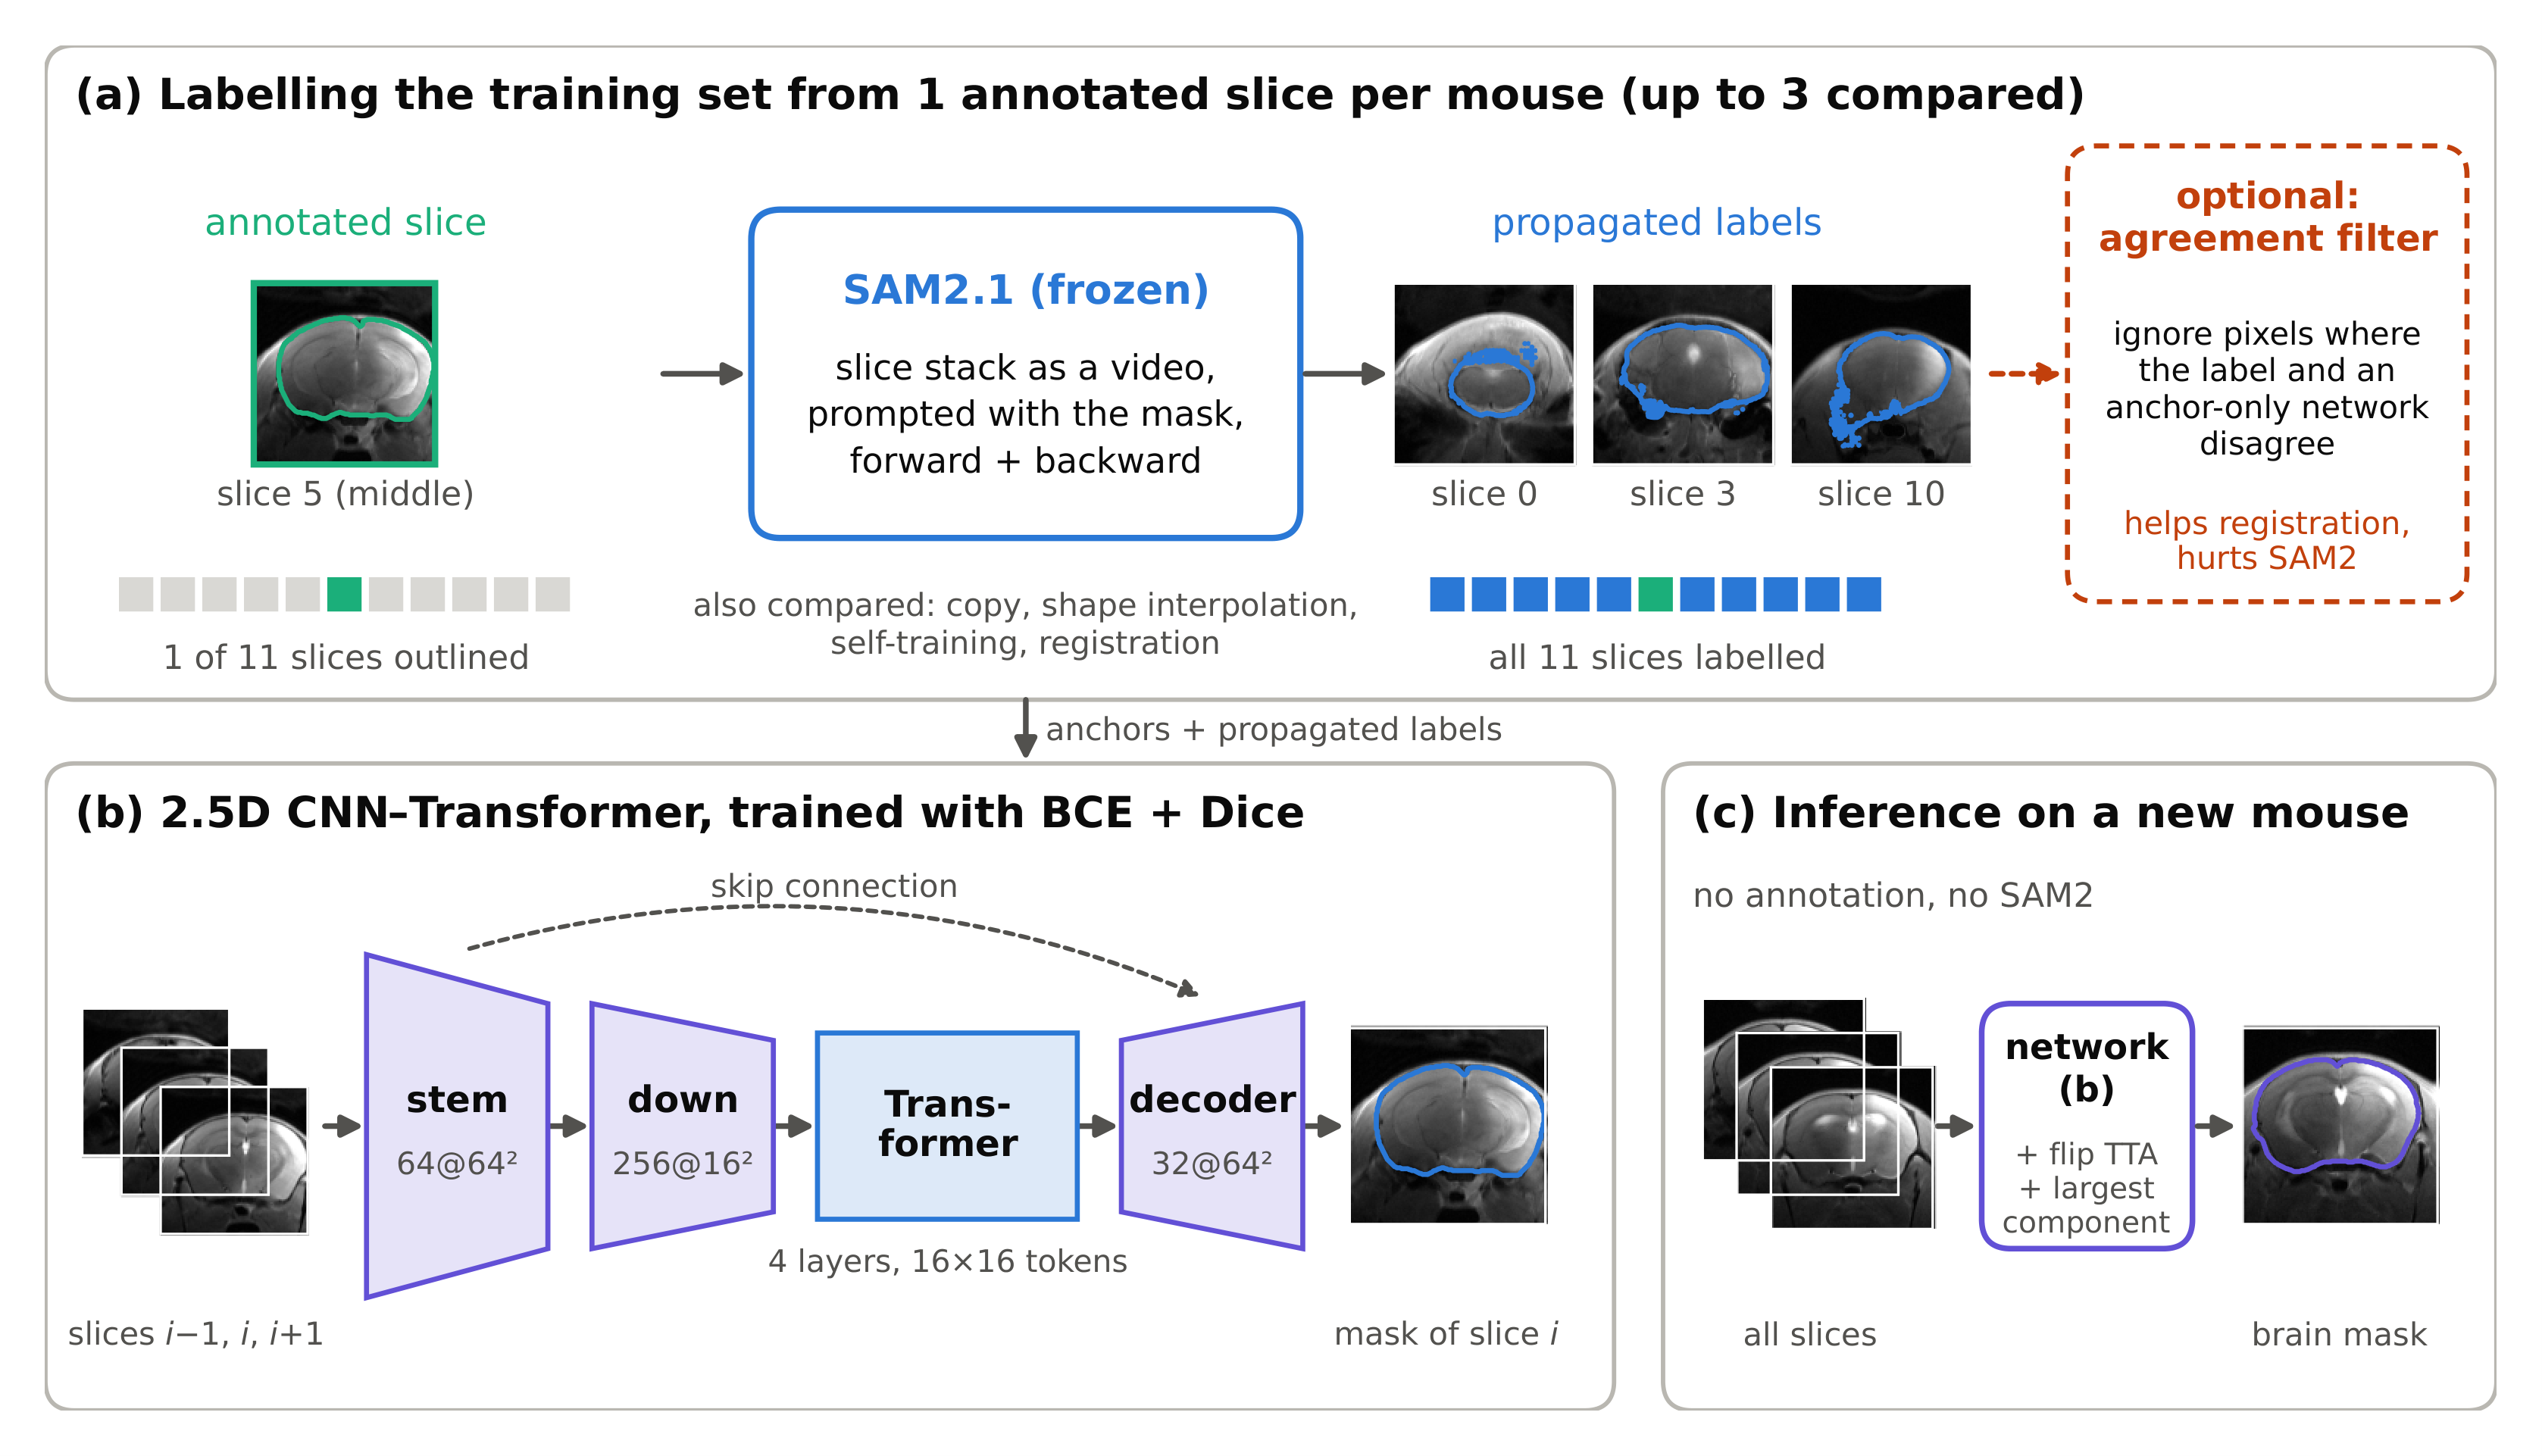
\includegraphics[width=0.84\linewidth]{fig_architecture.png}
\caption{Overview of the proposed workflow. (a) One to three slices from each training mouse are manually annotated (one slice is shown here). SAM2 uses these annotations to generate masks for the remaining slices. We also investigate an optional agreement-filtering step using a network trained only on the annotated slices. (b) The segmentation network takes three neighbouring slices as input. Two stride-2 convolutions in the stem, followed by two additional downsampling convolutions, produce a $16\times16$ grid of 256-dimensional tokens. These are processed by a four-layer Transformer, and a decoder with a skip connection from the stem predicts the mask of the centre slice. (c) Once trained, the network segments new mice without requiring manual annotations or SAM2.}
\label{fig:overview}
\end{figure*}

\subsection{Data and preprocessing}

We used an in-house MRI dataset containing 20 mice scanned with a 9.4~T Bruker small-animal scanner. The dataset includes axial T1- and T2-weighted images acquired with a slice thickness of 1~mm and a field of view of $14\times14$~mm. Each mouse has 10 or 11 slices, giving a total of 218 slices, all with expert-annotated brain masks.

The mice belong to two acquisition cohorts of ten animals each. Images in the first cohort have a matrix size of $256\times256$, while those in the second have a matrix size of $200\times200$. For preprocessing, we clipped the intensity values of each volume at the 0.5th and 99.5th percentiles, normalised them to $[0,1]$, and resampled all images to $256\times256$.

\subsection{Sparse annotation}

To investigate how much manual annotation is needed, we treated only one to three slices from each training mouse as annotated. We refer to these manually labelled slices as anchors, which are used to generate labels for the remaining slices.

For the main comparison of propagation methods, we selected three anchors per mouse. In the default arrangement, these were placed at indices $\lfloor n/4\rfloor$, $\lfloor n/2\rfloor$, and $\lfloor 3n/4\rfloor$, where $n$ is the number of slices in the volume. This arrangement leaves two slices at either end of the stack outside the outermost anchors.

We also examined a second arrangement, with anchors at indices $1$, $\lfloor n/2\rfloor$, and $n-2$. Here, the end slices are immediately adjacent to an annotated slice, reducing the distance over which labels must be extrapolated. Both arrangements use 60 annotated slices out of 218 (28\%).

We then reduced the annotation budget further to determine whether fewer anchors would be sufficient. For two-anchor experiments, we selected slices at $\lfloor n/3\rfloor$ and $\lfloor 2n/3\rfloor$, corresponding to 18\% of the dataset. For the single-anchor setting, only the middle slice, $\lfloor n/2\rfloor$, was annotated, reducing the proportion to 9\%.

Full manual masks were retained for the validation and test mice, but these were used only for model selection and performance evaluation.

\subsection{Segmentation network}

To ensure a fair comparison, all methods used the same 2.5D CNN--Transformer segmentation network (Fig.~\ref{fig:overview}b). The network takes three consecutive slices as input: the slice being segmented and its two immediate neighbours. These are combined as a three-channel input, allowing the model to use information from adjacent slices while predicting a mask for the centre slice.

The network was trained using an equally weighted combination of binary cross-entropy and soft Dice loss. Both losses were calculated over pixels with nonzero training weights, allowing uncertain labels to be excluded in the agreement-filtering experiments (Sec.~\ref{sec:agree}).

Training was performed for 8000 iterations using AdamW with an initial learning rate of $3\times10^{-4}$, cosine learning-rate decay, and a batch size of 8. Data augmentation included random rotations of up to $\pm15^\circ$, scaling by $\pm10\%$, horizontal flipping, and gamma augmentation. For each run, we selected the checkpoint with the highest validation Dice score.

During inference, we averaged the predictions from the original image and its horizontally flipped version. We then retained the largest connected component and filled any remaining holes to obtain the final brain mask. Importantly, once the network is trained, it can segment a new mouse without requiring an annotated slice or an additional SAM2 prompt.

\subsection{Propagators}
\label{sec:prop}

\textbf{SAM2.}
We treated each mouse MRI volume as a sequence of video frames, with individual slices representing consecutive frames. We used SAM2.1 (Hiera-L) \cite{ravi2024sam2} without any fine-tuning. The manually annotated anchor masks were provided as prompts, and SAM2 propagated them in both forward and backward directions through the slice stack. We averaged the probability maps from the two directions to obtain the final propagated labels.

\textbf{Registration with anchor consistency.}
As an alternative to SAM2, we used a U-Net to estimate dense displacement fields $\phi_{i\to j}$ between neighbouring slices, where $j=i\pm1$. The network operates at half the original image resolution and was trained using all neighbouring slice pairs from the training mice.

The registration objective combines local normalised cross-correlation, computed with a window size of 9, and a squared-gradient smoothness penalty on the displacement fields.

We additionally introduced an anchor-consistency loss to make use of the available sparse annotations. The idea is that a mask propagated from one annotated slice should align with the manual mask at the next annotated slice. To enforce this, we composed the displacement fields between two consecutive anchors, $a$ and $b$, and measured the Dice overlap between the warped mask and the target anchor mask:

\begin{equation}
\mathcal{L}_{\text{anchor}} =
1 - \operatorname{Dice}\!\left(
M_a \circ \phi_{a\to a\pm1}
\circ \dots \circ \phi_{b\mp1\to b},
\; M_b
\right).
\end{equation}

For each unannotated slice, we propagated masks from the nearest anchors on both sides and combined them using weights inversely proportional to the slice distance.

To assess the contribution of anchor consistency, we also evaluated registration without $\mathcal{L}_{\text{anchor}}$. Registration and the other baseline propagation methods were evaluated using three anchors per mouse.

\textbf{Baselines.}
We included three additional methods for comparison. The simplest approach copies the mask from the nearest annotated slice to each unannotated slice. Shape-based interpolation \cite{raya1990shape} instead interpolates signed distance maps between neighbouring anchors and extrapolates them beyond the outermost anchors.

We also evaluated self-training \cite{bai2017semi}. In this approach, a segmentation network is first trained using only the annotated slices. Its predictions on the remaining slices are then used as labels for training the final network.

\subsection{Self-supervised pretraining}
\label{sec:ssl}

As an alternative to propagation, we pretrained the segmentation encoder with masked image modelling, the approach of our previous work \cite{ali2025ssl}, on all slices of the training mice without their masks. Pretraining used AdamW with a learning rate of $5\times10^{-4}$ and a batch size of 8 for 4000 iterations. We then attached a new decoder and fine-tuned the complete network on the annotated slices only, with all parameters trainable.

\subsection{Agreement filtering}
\label{sec:agree}

Automatically propagated labels may contain errors, particularly in slices where brain anatomy differs substantially from the annotated anchors. We therefore investigated whether agreement with a separately trained segmentation network could help identify unreliable labels.

We first trained a network using only the manually annotated anchor slices. This network served as a teacher, providing predictions based on the image appearance rather than the propagation process.

For each unannotated pixel, we compared the teacher prediction with the propagated label. When both agreed, the propagated label was retained for training. When they disagreed, the pixel was assigned a loss weight of zero, so it did not contribute to the training objective.

For registration, the retained label was the average of the registration probability map and the teacher prediction. For SAM2, we retained SAM2's original label wherever the two methods agreed.

Finally, we trained a new segmentation network from scratch using the manually annotated anchors together with the propagated labels, applying the agreement-based weights where appropriate.


\subsection{Evaluation}

We evaluated all methods using five-fold cross-validation at the animal level, with the folds stratified by acquisition cohort. In each fold, 14 mice were used for training, two for validation, and four for testing, with two test mice selected from each cohort. This ensured that every mouse appeared in the test set exactly once. We repeated each fold with three random seeds to account for variability in training.

Performance was measured on all slices of the test mice using volumetric Dice and the mean slice-wise 95th-percentile Hausdorff distance (HD95), reported in pixels at a resolution of $256\times256$. For each mouse, we first averaged the results across the three seeds. We then compared methods using paired Wilcoxon signed-rank tests across the 20 mice.

To determine whether sparse annotation could achieve performance comparable to full annotation, we performed a one-sided paired Wilcoxon non-inferiority test with a margin of 0.01 Dice. This margin was approximately 2.4 times the mean seed-to-seed standard deviation (0.004) observed for the fully annotated network on an individual mouse. We also assessed the quality of the automatically propagated labels by comparing them with the withheld manual masks of the unannotated training slices.

We further examined how well the methods generalised across acquisition cohorts. For this experiment, we trained on eight mice from one cohort, used the remaining two for validation, and tested on all ten mice from the other cohort. We repeated the experiment in both directions, using three random seeds for each setting.

Finally, we evaluated whether the benefits of label propagation extended to a different segmentation architecture. We used nnU-Net v2 \cite{isensee2021nnunet} in its 2D configuration, keeping the default settings except for reducing training to 250 epochs. We trained nnU-Net once per fold on the same 14 training mice under three annotation settings: full annotation, one annotated slice per mouse supplemented with SAM2-propagated labels, and one annotated slice per mouse alone. In the last setting, all remaining slices were marked as ignored during training. For evaluation, we used the final checkpoint and applied the same post-processing procedure as for our CNN--Transformer network.

\section{Results}
\label{sec:results}

\begin{table}[t]
\centering
\caption{Test results on 20 mice (five-fold animal-level cross-validation, three seeds) with three annotated slices per training mouse at $n/4$, $n/2$, $3n/4$. Label: Dice of propagated labels on unannotated training slices. $^{*}$: different from anchors only ($p<0.05$). $^{\dagger}$: not different from full annotation ($p>0.05$). Dice standard deviations over mice were 0.02 to 0.04.}
\label{tab:results}
\small
\setlength{\tabcolsep}{3pt}
\begin{tabular}{@{}lccc@{}}
\toprule
Method & Dice $\uparrow$ & HD95 $\downarrow$ & Label \\
\midrule
Anchors only & 0.924 & 13.2 & -- \\
+ copy nearest & 0.908$^{*}$ & 13.3 & 0.864 \\
+ shape interpolation & 0.909$^{*}$ & 12.8 & 0.871 \\
+ self-training & 0.927$^{*}$ & 12.6 & 0.893 \\
+ registration & 0.930 & 11.7 & 0.902 \\
+ reg., anchor loss & 0.931$^{*}$ & 11.2 & 0.906 \\
+ reg., anchor loss, agreement & 0.933$^{*}$ & 11.0 & 0.911 \\
+ SAM2 & \textbf{0.950}$^{*\dagger}$ & \textbf{8.9} & \textbf{0.940} \\
+ SAM2, agreement & 0.940$^{*}$ & 10.5 & 0.940 \\
\midrule
All slices annotated & 0.946 & 9.0 & -- \\
\bottomrule
\end{tabular}
\end{table}

\begin{table}[t]
\centering
\caption{Annotation budget. Test Dice and HD95 (px) on 20 mice when training mice have one, two or three annotated slices, with the annotated slices alone or with SAM2-propagated labels, and with masked image pretraining at one slice. Label: Dice of SAM2 labels on unannotated slices. $^{\dagger}$: not different from the fully annotated model ($p>0.05$). Pretraining rows come from separate runs with the same folds, seeds and settings, and their own control (none).}
\label{tab:budget}
\small
\setlength{\tabcolsep}{3pt}
\begin{tabular}{@{}lcccccc@{}}
\toprule
 & & \multicolumn{2}{c}{Annotated only} & \multicolumn{3}{c}{+ SAM2} \\
\cmidrule(lr){3-4} \cmidrule(l){5-7}
Slices & \% & Dice & HD95 & Dice & HD95 & Label \\
\midrule
1 & 9 & 0.891 & 20.4 & \textbf{0.950}$^{\dagger}$ & 9.0 & 0.942 \\
2 & 18 & 0.925 & 13.4 & 0.949$^{\dagger}$ & 8.9 & 0.949 \\
3 & 28 & 0.924 & 13.2 & 0.950$^{\dagger}$ & 8.9 & 0.940 \\
All & 100 & 0.946 & 9.0 & -- & -- & -- \\
\midrule
\multicolumn{7}{@{}l}{One slice, pretraining instead of propagation:} \\
\multicolumn{2}{@{}l}{None} & 0.892 & 20.6 & & & \\
\multicolumn{2}{@{}l}{Masked modelling} & 0.890 & 21.4 & & & \\
\bottomrule
\end{tabular}
\end{table}

\begin{table}[t]
\centering
\caption{Second network and cohort shift. Test Dice and HD95 (px) with one slice alone, one slice plus SAM2 labels, or all slices annotated. nnU-Net: same 20 mice and folds, one run per fold. Cohort shift: our network trained on one cohort ($256\times256$ or $200\times200$) and tested on all ten mice of the other, three seeds. $^{\dagger}$: non-inferior to all slices at a 0.01 Dice margin ($p<0.01$).}
\label{tab:robust}
\small
\setlength{\tabcolsep}{2.5pt}
\begin{tabular}{@{}lcccccc@{}}
\toprule
 & \multicolumn{2}{c}{nnU-Net} & \multicolumn{2}{c}{$256\!\rightarrow\!200$} & \multicolumn{2}{c}{$200\!\rightarrow\!256$} \\
\cmidrule(lr){2-3} \cmidrule(lr){4-5} \cmidrule(l){6-7}
Annotation & Dice & HD95 & Dice & HD95 & Dice & HD95 \\
\midrule
One slice & 0.868 & 23.1 & 0.891 & 18.1 & 0.777 & 42.9 \\
+ SAM2 & 0.958$^{\dagger}$ & 7.6 & 0.929$^{\dagger}$ & 11.9 & 0.790 & 35.1 \\
All slices & \textbf{0.960} & \textbf{6.9} & \textbf{0.931} & \textbf{11.4} & \textbf{0.809} & \textbf{32.4} \\
\bottomrule
\end{tabular}
\end{table}

\begin{figure}[t]
\centering
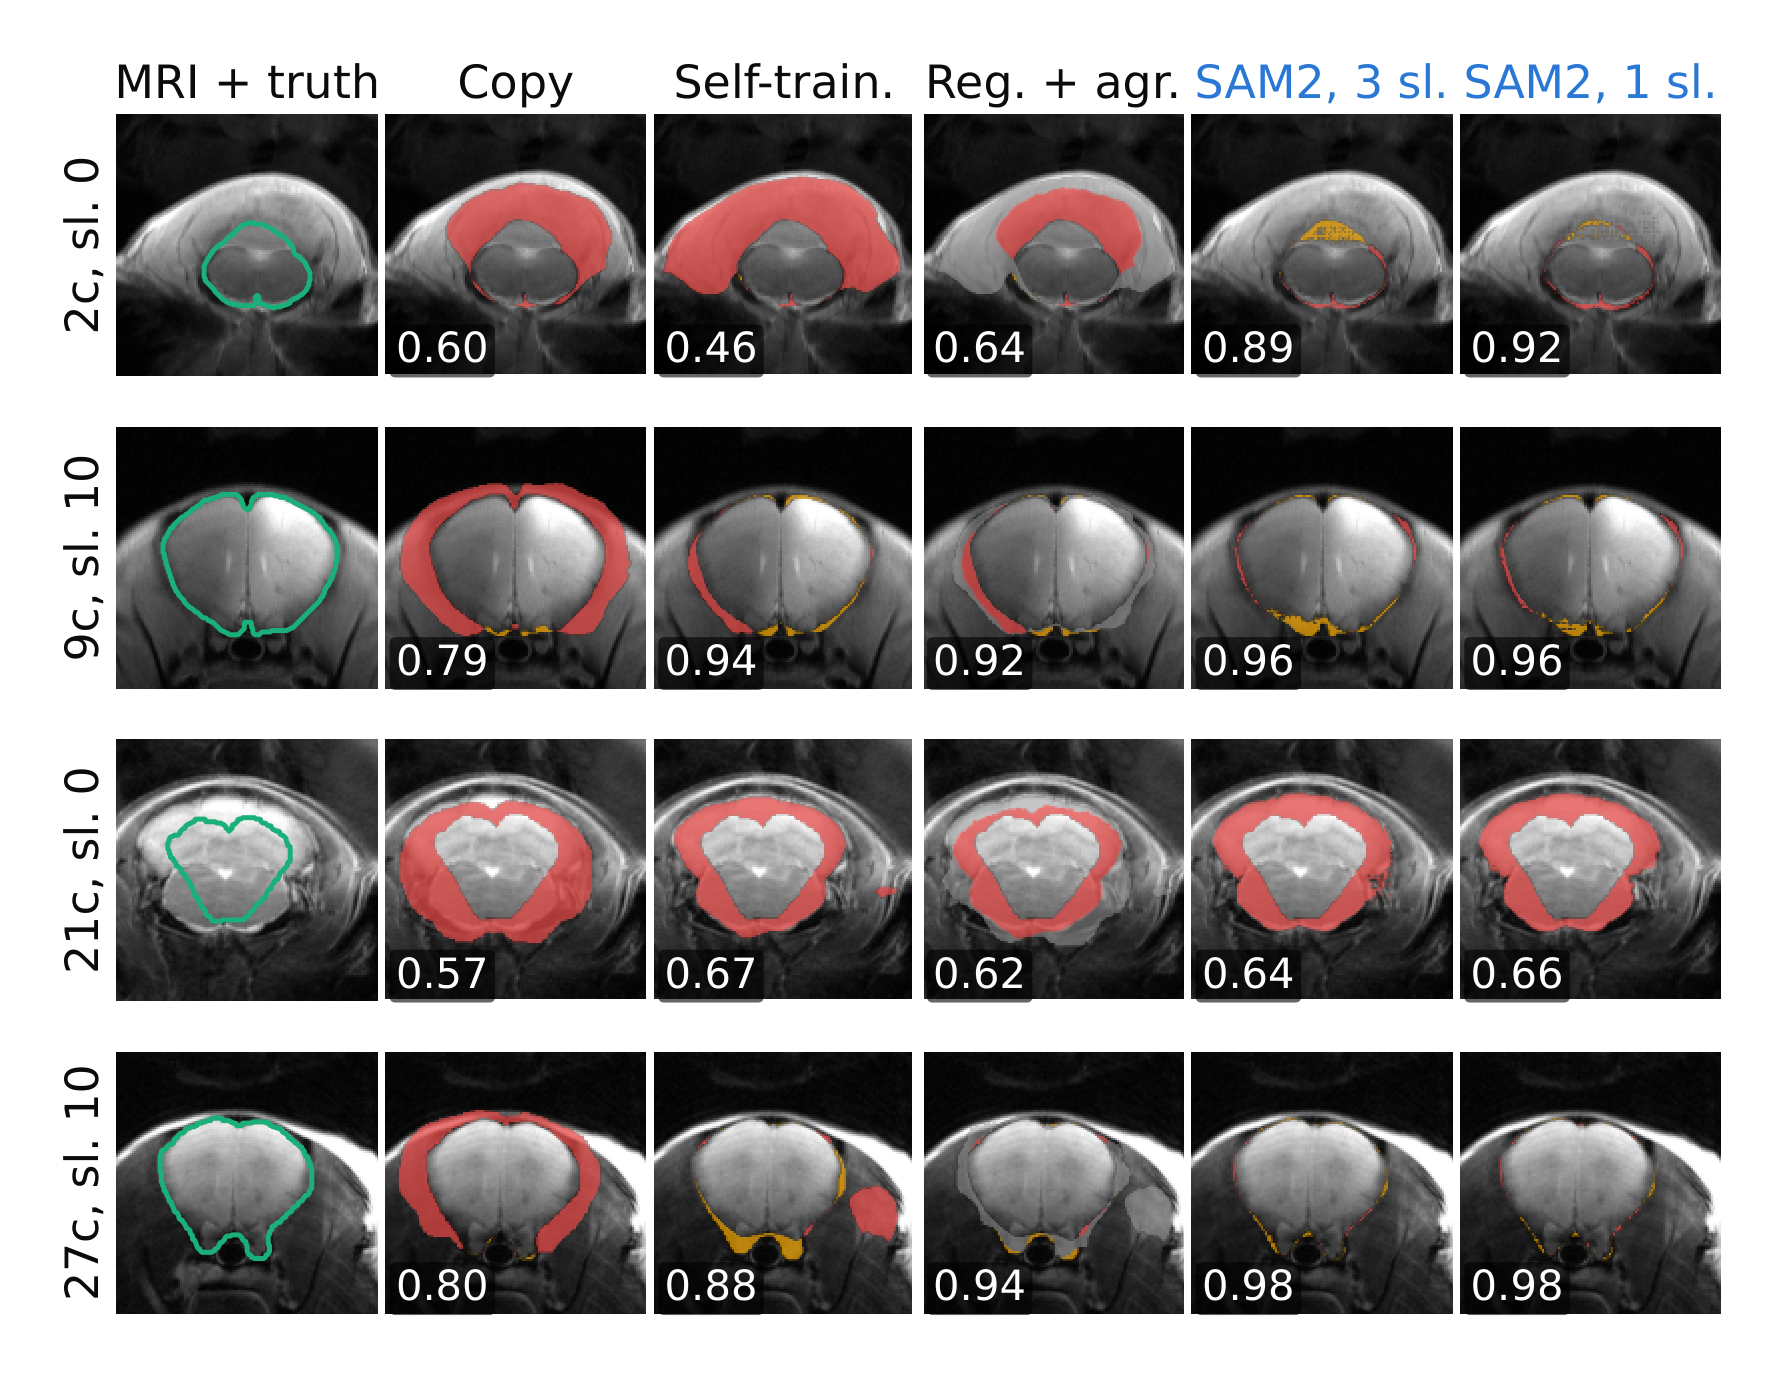
\includegraphics[width=\linewidth]{fig_qualitative_pseudo_labels.png}
\caption{Propagated labels on an end slice of four training mice (two per cohort), which lies beyond the outermost anchor. Columns 2--5 use three anchors, the last column SAM2 from the middle slice only. Numbers: label Dice. Green: ground truth. Red: false positive. Amber: false negative. Grey: excluded by agreement filtering.}
\label{fig:qualitative}
\end{figure}

\textbf{Three slices with SAM2 match full annotation.} Table~\ref{tab:results} lists test performance on unseen mice for the default anchor layout. Training on the three annotated slices alone reached a Dice of 0.924, against 0.946 when every slice was annotated ($p<0.001$). With SAM2-propagated labels, the network reached 0.950 and an HD95 of 8.9~px. It was better than the anchor-only network on 19 of 20 mice ($p<0.001$) and better than the best registration variant on 19 of 20 ($p<0.001$). It did not differ from the fully annotated network in Dice ($p=0.96$) or HD95 ($p=0.76$). The 95\% bootstrap confidence interval of the paired Dice difference was $-0.001$ to $0.009$, and the result held in both cohorts (0.956 and 0.944, against 0.953 and 0.940). SAM2 labels were weakest on two mice of the $200\times200$ cohort (0.79 and 0.81), which were also the hardest test cases for the fully annotated network.

\textbf{One slice is enough.} Table~\ref{tab:budget} reduces the budget. With only the middle slice annotated, the network trained on that slice alone fell to a Dice of 0.891 and an HD95 of 20.4~px ($p<0.001$ against full annotation). With SAM2 labels it reached 0.950 and 9.0~px, better than the single-slice network on all 20 mice ($p<0.001$) and non-inferior to full annotation ($p<0.001$ at a 0.01 margin, $p=0.001$ at 0.005). The paired difference had a mean of $+0.004$ but a median of $-0.001$: the network trained on SAM2 labels was better on 9 of 20 mice, by up to 0.07 on a mouse that was hard for the fully annotated network (0.905), and worse on 11 by at most 0.011 (95\% confidence interval $-0.002$ to $0.013$, HD95 $p=0.43$). Two and three slices were also non-inferior ($p<0.001$). The accuracy of SAM2 labels fell with distance from the annotated slice, from 0.976 on the adjacent slices to 0.880 five slices away, but the network trained on them did not inherit this loss. On the same slices (0, 4, 6 and 10, never an anchor in any layout), SAM2 labels from one, two and three anchors were equally accurate (0.925, 0.926 and 0.925; interior 0.975, end slices 0.877), so extra anchors did not improve SAM2 labels, and the higher overall label Dice with one anchor in Table~\ref{tab:budget} reflects which slices are scored. Applied directly to each test mouse with its middle slice annotated, SAM2 reached 0.956, but it needs an annotated slice for every new animal, whereas the trained network needs none.

\textbf{Naive propagation hurts.} Copying the nearest mask or interpolating signed distances lowered the test Dice to 0.908 and 0.909, below the anchor-only network. Their labels were accurate next to an anchor (0.92--0.93) but fell to 0.705 on the two end slices, where the brain narrows and no anchor bounds the extrapolation (Fig.~\ref{fig:qualitative}). Self-training labelled the end slices at 0.726 because the teacher leaks into skull and neck tissue. Registration held 0.786 there and SAM2 0.883.

\textbf{Agreement filtering depends on the propagator.} Filtering excluded 2--3\% of the unannotated pixels for every propagator. For registration it gave the best variant in both layouts (0.933 and 0.938), although the gain over the unfiltered labels was significant only in the second layout ($p=0.015$, against $p=0.6$). For SAM2 it reduced Dice from 0.950 to 0.940 ($p<0.001$, 18 of 20 mice) and raised HD95 from 8.9 to 10.5~px. Registration had labelled 57--60\% of them correctly, close to chance, so removing them removed mostly noise. SAM2 had labelled 72--78\% of them correctly, so filtering removed correct labels from the boundary, where supervision matters most for HD95.

\textbf{Placement of the annotated slices.} Moving the outer anchors next to the ends of the stack turns extrapolation into interpolation. It raised the anchor-only network (0.924 to 0.929, $p=0.007$), interpolation (0.909 to 0.918, $p<0.001$) and filtered registration (0.933 to 0.938, $p=0.001$), but not SAM2 (0.950 and 0.946, $p=0.11$), whose labels at the ends were already accurate.

\textbf{Pretraining does not replace propagation.} Masked image pretraining did not improve the single-slice network (0.890 against 0.892 without pretraining, Table~\ref{tab:budget}), and with three annotated slices it was slightly worse (0.922 against 0.925, $p<0.05$). It leaves the unannotated slices without supervision, which propagation provides.

\textbf{The result holds for nnU-Net.} With full annotation nnU-Net reached a Dice of 0.960 and an HD95 of 6.9~px (Table~\ref{tab:robust}), 0.013 above our network ($p<0.001$). Trained on SAM2 labels from one slice it reached 0.958 and was non-inferior to its fully annotated counterpart ($p<0.001$), better on 5 of 20 mice, with a slightly higher HD95 (7.6~px, $p=0.03$). Trained on the annotated slice alone it fell to 0.868, lower than our network on the same data (0.891, $p=0.002$). The benefit of propagation therefore does not depend on the segmentation network, and a stronger network gains at least as much from it (0.090 against 0.059).

\textbf{Shift between cohorts.} Training on one cohort and testing on the other lowered every method (Table~\ref{tab:robust}). From the $256\times256$ to the $200\times200$ cohort, one slice with SAM2 labels stayed non-inferior to full annotation (0.929 against 0.931, $p=0.005$), while the slice alone fell to 0.891. In the other direction all methods degraded strongly (full annotation 0.809 against 0.953 within the cohort), and SAM2 labels fell 0.019 below full annotation ($p=0.004$), so non-inferiority was not shown under this shift.

\section{Discussion and conclusion}
\label{sec:discussion}
One annotated slice per mouse and a promptable video model replaced full slice-by-slice annotation for training a brain extraction network, with 91\% fewer annotated slices and no loss in accuracy beyond a 0.01 Dice margin. Annotation time was not measured and need not scale with the slice count. SAM2 is needed only once, to label the training set, and the deployed network segments a new mouse without any annotation.

Two practical points follow. A propagator that cannot follow anatomy beyond the annotated slices is worse than none, because its errors at the ends of the brain repeat in every training mouse. Filtering labels by agreement with an anchor-trained network helps a propagator whose disputed pixels are close to chance and harms one whose disputed pixels are mostly correct.

The study has limits. The dataset has 20 mice from one scanner, the slices are 1~mm thick and the evaluation covers whole-brain masks only. Checkpoints were selected on two fully annotated validation mice per fold, an annotation cost that a deployment with one slice per mouse would also carry. Under the stronger of the two cohort shifts, one slice was not enough, so the result should be confirmed on each new protocol. Our network was not tuned for accuracy, and nnU-Net was better with full or propagated labels. Pretraining used only the slices of the training mice, and pretraining on larger unlabelled archives may behave differently.

\section{Compliance with ethical standards}
\label{sec:ethics}
\todo{Animal study approval: institution and protocol number (IACUC) for the MRI data, from coauthors.}

\section{Acknowledgments}
\label{sec:acknowledgments}
\todo{Funding sources; or state that no funding was received.} The authors have no relevant financial or non-financial interests to disclose.

\bibliographystyle{IEEEbib}
\bibliography{refs}

\end{document}
